%
%  exercise-2.tex
%  artificial intelligence
%
%  Created by Illya Starikov on 01/21/18.
%  Copyright 2018. Illya Starikov. All rights reserved.
%

\RequirePackage[l2tabu, orthodox]{nag}
\documentclass[12pt]{scrartcl}

\newcommand{\exercisenumber}{2}
\newcommand{\duedate}{January 24\textsuperscript{th}, 2018}

\usepackage{amssymb,amsmath,verbatim,graphicx,microtype,upquote,units,booktabs,akkwidepage}

\newcommand{\chapterNumber}[1]{
    \setcounter{section}{#1}
    \addtocounter{section}{-1}
}
\newcommand{\statedescript}{\left(C_L,\, M_L,\, B_{L/R}\right)}

\newcommand{\cannibal}{\textcolor{red}{Cannibal}}
\newcommand{\missionary}{\textcolor{purple}{Missionary}}

\begin{document}
\maketitle

For these problems, we split the river into two sections into two section: Left and Right. Left is assumed to be the initial state.

\section{Problem Formulation}
\begin{statement}
    Precisely formulate the problem.
\end{statement}

\begin{enumerate}
    \item A method of describing a state would be with the tuple: $\statedescript$, where:
        \begin{align*}
            C_L     &= \text{The number of Cannibals on the Left} \\
            M_L     &= \text{The number of Missionaries on the Left} \\
            B_{L/R} &= \text{The location (Left/Right) of the boat}
        \end{align*}

        However, we restrict these numbers to as follows:

        We do not care about the number of Cannibals/Missionaries on the right, because we can calculate them as follows:
        \begin{equation*}
            C_R = 3 - C_L \qquad M_R = 3 - M_L
        \end{equation*}

        Although these values are not strictly within the state description, from here forth (for readability purposes) we act as if it is, mentally replacing $C_R$ and $M_R$ with these values. The final desciption is still $\statedescript$, and these are merely computed properties of the state.

        Note, however, because we want to restrict our state space to only valid states, we place the following restrictions:
        \begin{equation*}
            M_L \geq C_L \quad\textbf{and}\quad M_R \geq C_R
        \end{equation*}

        Furthermore,

        \begin{equation*}
            B_{L/R} = \text{Left} \iff M_L + B_L = 6 \qquad B_{L/R} = \text{Right} \iff M_R + B_R = 6
        \end{equation*}

    \item The initial state is as follows:
        \begin{equation*}
            \statedescript = \left(3,\, 3,\, L\right)
        \end{equation*}

    \item Our $\textsc{ACTIONS}$ are defined as follow. We use synonyms $L \leftrightarrow \text{Left}$ and $R \leftrightarrow \text{Right}$.

        Basically, we check to see if we can send one of both \cannibal{} and \missionary{}. If we can, add them to the solution set. Next, we check to see if we can send either \num{1} \cannibal{} and \num{1} \missionary{}. After, we check to see if we can send \num{2} \cannibal{} and \num{2} \missionary{}. Because there are rules we have to account for (i.e., there must be more \missionary{} than \cannibal{} \textit{unless there's 0 \missionary{}}).
\end{enumerate}

\begin{algorithmic}[1]
    \Statex{}
    \Function{$\neg$}{direction}
        \If{$\text{direction} = \text{Left}$}
            \State{\Return{Right}}
        \Else{}
            \State{\Return{Left}}
        \EndIf{}
    \EndFunction{}
    \State{}\State{}

    \Function{Actions}{$s$}
        \Let{PossibleActions}{$\{\}$} \Comment{A set \textit{of sets} of moves}
        \State{}

        \ForAll{$\text{direction } d \in \{\text{Left}, \text{Right}\}$}
            \If{$a.M_d > 0 \textbf{ and } a.C_d > 0$}
                \Let{NewAction}{$\{\text{send \cannibal{} $d$ \textrightarrow{} $\neg{d}$}\}$}
                \Let{NewAction}{$\{\text{send \missionary{} $d$ \textrightarrow{} $\neg{d}$}\}$} \Comment{Note this has the form $\{ \ldots,\, \ldots \}$}
                \State{}

                \Let{PossibleActions}{$\text{PossibleActions } \cup \{\text{ NewAction}\}$} \Comment{Note this has the form $\{\ldots,\, \{ \ldots,\, \ldots \},\, \ldots \}$}
            \EndIf{}

            \State{}
            \For{$i \leftarrow 1 \textbf{ to } 2$}
                \If{$a.M_d - i \geq 0$} \Comment{Is there even enough missionaries to remove?}
                    \If{$\left(a.M_d - i \geq a.C_d \textbf{ or } a.M_d - i = 0 \right) \textbf{ and } a.M_{\neg{d}} + i \geq a.C_{\neg{d}}$}
                        \Let{NewAction}{$\{\text{send $i$ \missionary{} $d$ \textrightarrow{} $\neg{d}$ }\}$}\footnote{Note by saying ``send $i$ \missionary{}'', we are just saying ``send a missionary'' $i$ times. For $i = 2$, we have $\text{NewAction} \leftarrow \{ \text{send a missionary},\text{send a missionary} \}$.}
                        \Let{PossibleActions}{$\text{PossibleActions } \cup \{\text{ NewAction}\}$}
                    \EndIf{}
                \EndIf{}
                \State{}

                \If{$a.C_d - i \geq 0$} \Comment{Is there even enough cannibals to remove?}
                    \If{$a.C_{\neg{d}} + i \leq a.M_{\neg{d}} \textbf{ or } a.M_{\neg{d}} = 0$}
                        \Let{NewAction}{$\{\text{send $i$ \cannibal{} $d$ \textrightarrow{} $\neg{d}$}\}$}\footnote{See previous footnote.}
                        \Let{PossibleActions}{$\text{PossibleActions } \cup \{\text{ NewAction}\}$}
                    \EndIf{}
                \EndIf{}

            \EndFor{}
        \EndFor{}

        \State{}
        \State{\Return{PossibleActions}}
    \EndFunction{}
\end{algorithmic}

\begin{enumerate}
    \setcounter{enumi}{3}
    \item We define $\textsc{Results}(s,\, a)$ as follows.
\end{enumerate}

\begin{algorithmic}[1]
    \Function{Results}{s,\, a}
        \Let{$a'$}{$a$}

        \State{$a'.B_{L/R} = \neg{a'.B_{L/R}}$}
        \State{}

        \ForAll{$\text{action} \in a$} \Comment{We defined an action as a set of steps}
            \If{$\text{action} = \text{send \cannibal{} Left \textrightarrow{} Right}$}
                \State{$a'.C_L = a'.C_L - 1$}
            \EndIf{}

            \State{}
            \If{$\text{action} = \text{send \cannibal{} Right \textrightarrow{} Left}$}
                \State{$a'.C_L = a'.C_L + 1$}
            \EndIf{}

            \State{}
            \If{$\text{action} = \text{send \missionary{} Left \textrightarrow{} Right}$}
                \State{$a'.M_L = a'.M_L - 1$}
            \EndIf{}

            \State{}
            \If{$\text{action} = \text{send \missionary{} Right \textrightarrow{} Left}$}
                \State{$a'.M_L = a'.M_L + 1$}
            \EndIf{}
        \EndFor{}

        \State{}
        \State{\Return{$a'$}}
    \EndFunction{}
\end{algorithmic}

\begin{enumerate}
    \setcounter{enumi}{4}
    \item We define $\textsc{IsGoal}(s)$ as follows.
\end{enumerate}

\begin{algorithmic}[1]
    \Function{IsGoal}{$s$}
        \State{\Return{$s = \left(0,\, 0,\, \text{Right}\right)$}}
    \EndFunction{}
\end{algorithmic}

\begin{enumerate}
    \setcounter{enumi}{5}
    \item We define $\textsc{C}(s,\, a,\, s')$
\end{enumerate}

\begin{algorithmic}[1]
    \Function{C}{$s,\, a,\, s'$}
        \State{\Return{|a|}}\footnote{We define the $|x|$ operator to return the length of $x$.}
    \EndFunction{}
\end{algorithmic}

\section{State Space}
Figure~\ref{fig:state_space} provides the complete space for the problem, with \textcolor{purple}{M} representing Missionaries and \textcolor{red}{C} representing cannibals.

\begin{figure}[htpb]
    \centering
    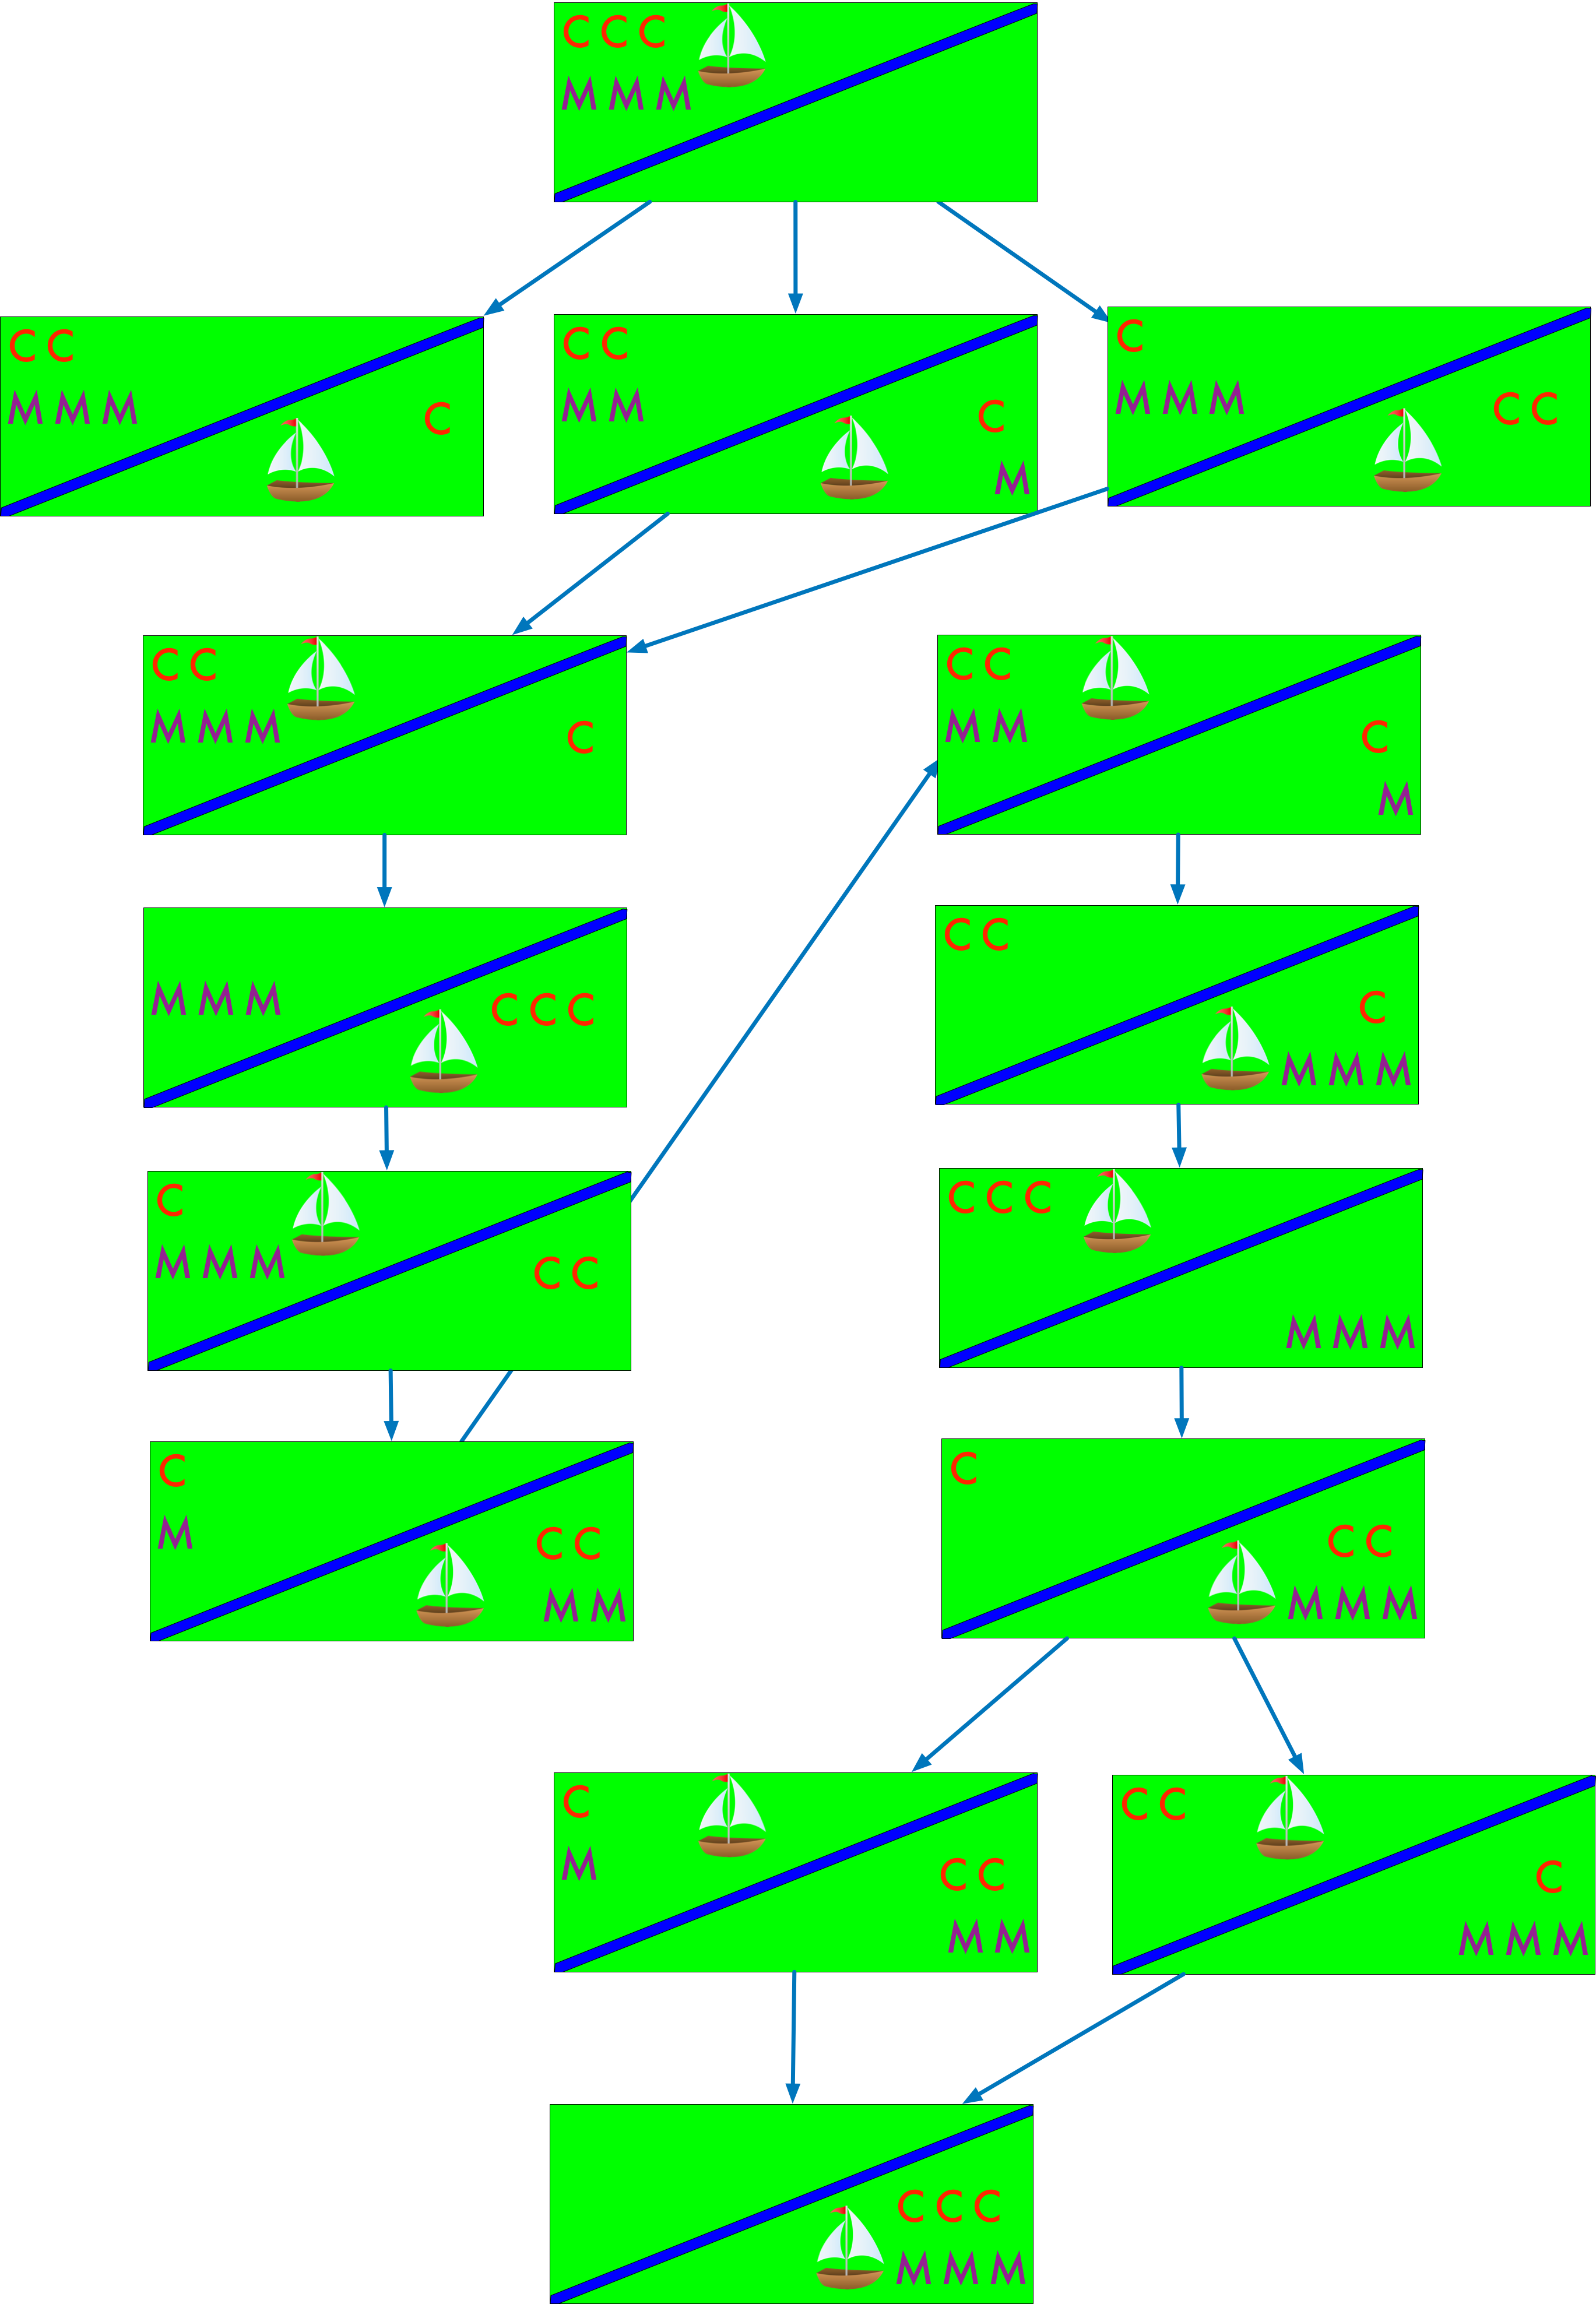
\includegraphics[width=.9\textwidth]{./assets/2.1-diagram.png}
    \caption{The Complete State Space}\label{fig:state_space}
\end{figure}

\section{Possible Solution}
Figure~\ref{fig:success} outlines a path for a solution, with \textcolor{purple}{M} representing Missionaries and \textcolor{red}{C} representing cannibals.

\begin{figure}[htpb]
    \centering
    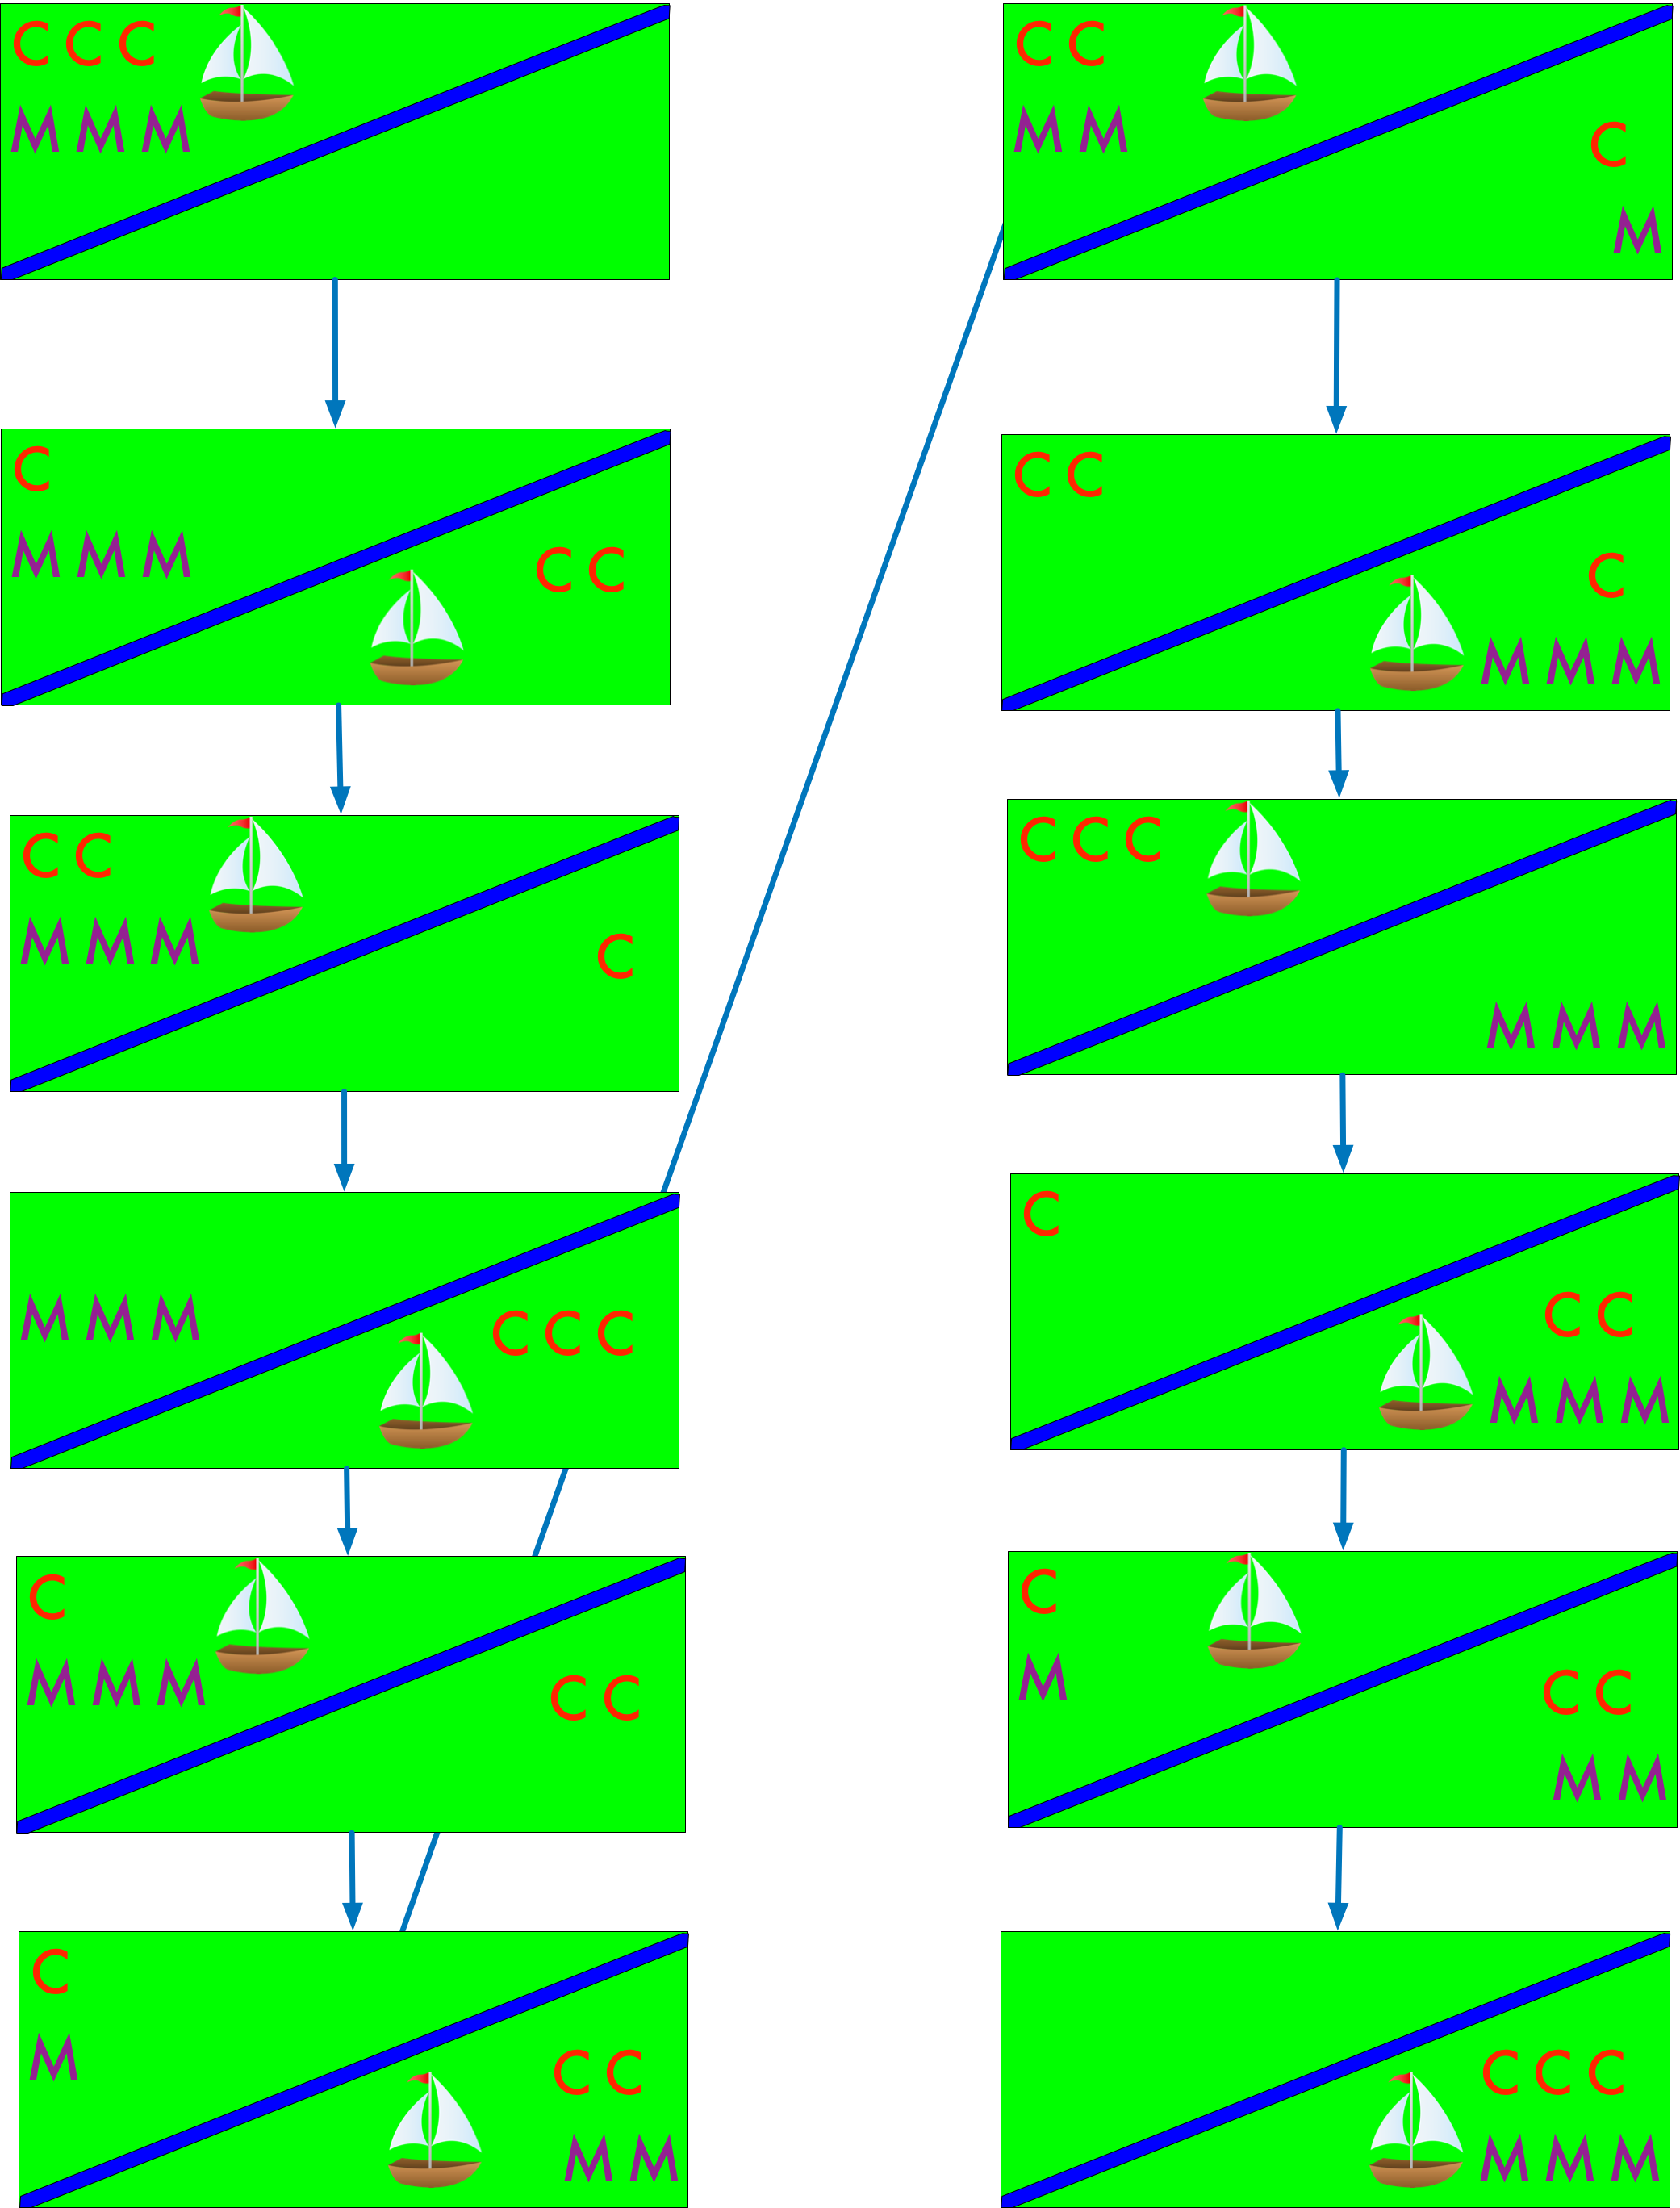
\includegraphics[width=.9\textwidth]{./assets/2.2-diagram.png}
    \caption{Path To A Solution}\label{fig:success}
\end{figure}

\end{document}
